\section{Validation Strategy and Quantitative Accuracy}
\label{sec:numerical_protocol}

\paragraph{Validation philosophy.}
The goal is targeted falsification of the representative maps, not broad numerical benchmarking.
Each diagnostic is tied directly to one physical claim:
(i) involutive branch exchange,
(ii) orientation-gauge affine reflection,
and (iii) quantitative usefulness of asymptotic reconstruction away from crossover.

\subsection{Core branch-exchange visualization}

\begin{figure*}[t]
  \centering
  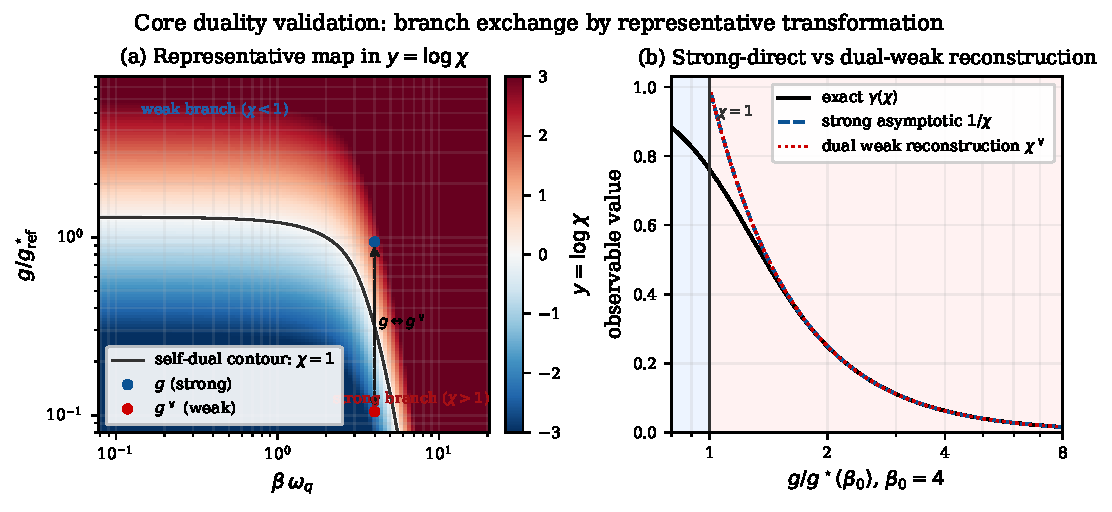
\includegraphics[width=0.86\textwidth]{../figures/hmf_dual_map_core.pdf}
  \caption{
  Core dual-representative validation.
  \textbf{(a)} Map of \(y=\log\chi\) in \((\beta,g)\), with self-dual contour \(\chi=1\), branch
  labels, and a fixed-\(\beta\) pair \(g\leftrightarrow g^\vee\).
  \textbf{(b)} At fixed \(\beta_0\), direct \(\gamma(\chi)\), strong asymptotic \(1/\chi\), and dual
  weak variable \(\chi^\vee\). Their convergence on \(g/g^\star>1\) visualizes branch-transfer
  control.
  }
  \label{fig:core_dual_map_v2}
\end{figure*}

\subsection{How accurate is the analytic reconstruction?}

\begin{figure}[tbp]
  \centering
  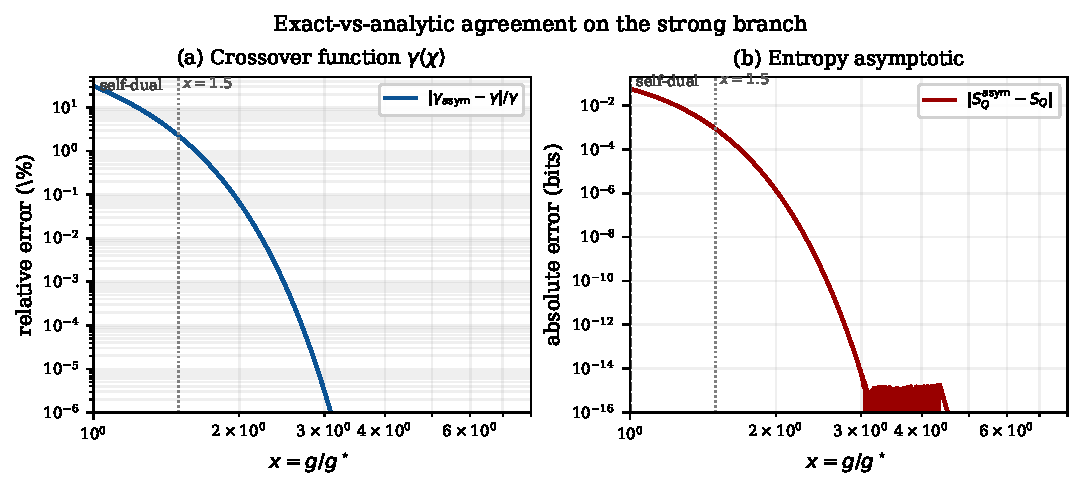
\includegraphics[width=\columnwidth]{../figures/hmf_exact_vs_analytic_error.pdf}
  \caption{
  Exact-vs-analytic error diagnostics on the strong branch \(x:=g/g^\star\ge1\).
  \textbf{(a)} Relative error of \(\gamma_{\mathrm{asym}}=1/\chi\) versus
  \(\gamma_{\mathrm{exact}}=\tanh\chi/\chi\) with \(\chi=x^2\).
  \textbf{(b)} Absolute entropy error in bits for
  \(S_Q^{\mathrm{asym}}=((1+2\chi)e^{-2\chi})/\ln2\) versus
  \(S_Q^{\mathrm{exact}}=h_2((1+|\tanh\chi|)/2)\).
  The dominant mismatch is confined to the immediate crossover neighborhood.
  }
  \label{fig:exact_vs_analytic_error_v2}
\end{figure}

\begin{table}[tbp]
  \caption{Agreement windows for \(x\ge x_{\min}\).
  \(\delta_\gamma:=|\gamma_{\mathrm{asym}}-\gamma_{\mathrm{exact}}|/\gamma_{\mathrm{exact}}\),
  \(\Delta S_Q:=S_Q^{\mathrm{asym}}-S_Q^{\mathrm{exact}}\).
  Entries for \(\delta_\gamma\) are percentages; entries for \(|\Delta S_Q|\) are bits.}
  \label{tab:exact_vs_analytic_metrics_v2}
  \begin{ruledtabular}
  \begin{tabular}{ccccc}
    \(x_{\min}\) & \(\max \delta_\gamma\) & \(\mathrm{RMS}\,\delta_\gamma\) & \(\max|\Delta S_Q|\) & \(\mathrm{RMS}\,|\Delta S_Q|\) \\
    \hline
    1.0 & 31.30\% & 6.68\% & \(5.87\times10^{-2}\) & \(1.08\times10^{-2}\) \\
    1.2 & 11.87\% & 2.33\% & \(1.45\times10^{-2}\) & \(2.30\times10^{-3}\) \\
    1.5 & 2.24\% & 0.389\% & \(8.79\times10^{-4}\) & \(1.16\times10^{-4}\) \\
    2.0 & 0.0668\% & 0.00978\% & \(1.37\times10^{-6}\) & \(1.48\times10^{-7}\) \\
  \end{tabular}
  \end{ruledtabular}
\end{table}

\paragraph{Interpretation.}
The asymptotic reconstruction is intentionally not expected to be accurate exactly at
self-duality \(x\approx1\).
What matters for control transfer is performance in the target branch.
By \(x\ge1.5\), \(\gamma\) errors are already at the few-percent level and entropy errors are
sub-millibit.
By \(x\ge2\), the reconstruction is effectively exact at manuscript resolution.

\subsection{Minimal acceptance checks}

\begin{enumerate}
  \item Involution: \((g^\vee)^\vee=g\) and
  \(\chi(\beta,g^\vee,\theta)=1/\chi(\beta,g,\theta)\).
  \item Orientation: \(\beff'+\beff=2\beta\), with radial invariants unchanged.
  \item Asymptotic transfer: direct strong-branch evaluation agrees with dual weak-branch
  reconstruction in the intended window.
  \item Manuscript consistency: figure scripts, table values, and text-level claims are synchronized.
\end{enumerate}

\paragraph{Reproducibility note.}
Core and comparison assets are produced by the project validation scripts.
The quantitative table values are taken from the generated metrics CSV in the same validation
pipeline.
